
使用CMake最常见的方式是通过命令行(CLI)。本节中,将了解如何使用CLI执行最基本的CMake操作。

与CMake CLI的交互可以通过在终端中输入CMake命令来完成,假设安装了CMake,并且CMake可执行文件包含在系统的PATH变量(或等效变量)中。就可以通过在终端中直接使用cmake进行验证:

\begin{center}
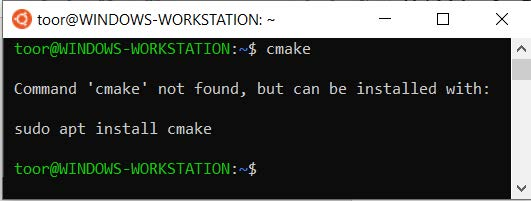
\includegraphics[width=0.6\textwidth]{content/1/chapter2/images/1.jpg}\\
图2.1 使用cmake命令
\end{center}

若终端抱怨缺少命令,需要安装CMake或者将其可执行文件的目录添加到系统的PATH环境变量中。关于如何向系统的PATH变量添加路径,请参考操作系统指南。

在安装CMake并将其添加到PATH变量后(如果需要),需要测试CMake是否可用。可以在命令行中执行\texttt{cmake -{}-version},检查CMake版本。

\begin{center}
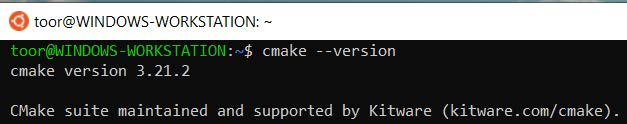
\includegraphics[width=0.6\textwidth]{content/1/chapter2/images/2.jpg}\\
图2.2 终端中查看CMake版本
\end{center}

CMake版本将以<maj.min.rev>的形式输出。

\begin{tcolorbox}[colback=webgreen!5!white,colframe=webgreen!75!black,title=Note]
若版本与安装的不匹配,可能系统中安装了多个CMake。由于本书包含了为CMake 3.21及以上版本编写的示例,因此建议在进一步深入前修复该问题。
\end{tcolorbox}

安装CMake之后,应该安装构建系统和编译器。对于类似Debian的操作系统(例如,Debian和Ubuntu),这可以通过\texttt{sudo apt install build-essential}命令轻松完成,包含对gcc、g++和make的安装。

CLI的用法将在Ubuntu 20.04环境中说明,在其他环境中的用法也相同。

\subsubsubsection{2.2.1\hspace{0.2cm}了解CMake命令行的基本操作}

下面列出了使用CMake命令行应该了解的三件事:

\begin{itemize}
\item 
配置

\item 
构建

\item 
安装
\end{itemize}

学习了基础知识之后,将能够构建和安装CMake项目。

\hspace*{\fill} \\ %插入空行
\noindent
\textbf{通过命令行配置项目}

要通过命令行配置CMake项目,可以使用\texttt{CMake -G "Unix Makefiles" -S  -B <output\_directory>}的方式。-S参数用于指定要配置的CMake项目,而-B参数用于指定配置输出目录。最后,-G参数指定将用于生成构建系统的生成器,配置过程的结果将写入<output\_directory>。

在项目根构建目录中配置我们书中的示例项目:

\begin{center}
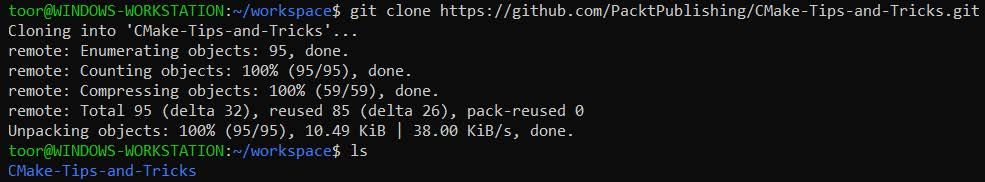
\includegraphics[width=0.8\textwidth]{content/1/chapter2/images/3.jpg}\\
图2.3 克隆示例代码存储库
\end{center}

\begin{tcolorbox}[colback=webgreen!5!white,colframe=webgreen!75!black,title=重要Note]
项目必须存在于环境中。若没有,需要在Git在终端中执行\texttt{git clone \url{https://github.com/PacktPublishing/CMake-Best-Practices.git}}。
\end{tcolorbox}

现在进入CMake-Best-Practices目录,使用\texttt{cmake -G "Unix Makefiles" -S . -B ./build}:

\begin{center}
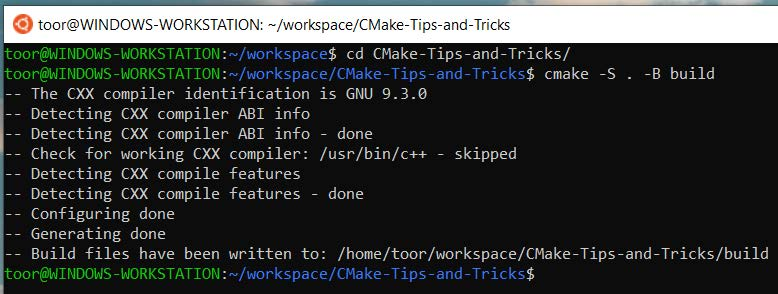
\includegraphics[width=0.8\textwidth]{content/1/chapter2/images/4.jpg}\\
图2.4 使用CMake配置示例代码
\end{center}

使用"Unix Makefiles" (\texttt{-G "Unix Makefiles"})生成器在当前目录(\texttt{-S .})生成CMake项目的构建系统(\texttt{-B ./build})目录。

CMake将设置源文件夹为当前文件夹中的项目。当省略构建类型时,CMake使用Debug构建类型(项目默认的\texttt{CMAKE\_BUILD\_TYPE})。

后续章节中,我们将学习配置步骤中使用的基本设置。

\hspace*{\fill} \\ %插入空行
\noindent
\textbf{修改构建类型}

CMake不假定构建类型。为了设置构建类型,必须在配置阶段提供一个名为CMAKE\_BUILD\_TYPE的变量,变量必须以-D作为前缀。

要获得Release版本,而不是Debug版本,需要在配置命令中添加CMAKE\_BUILD\_TYPE变量,该命令为:\texttt{cmake -G "Unix Makefiles" -DCMAKE\_BUILD\_TYPE:STRING=Release -S . -B ./build}。

\begin{tcolorbox}[colback=webgreen!5!white,colframe=webgreen!75!black,title=Note]
\texttt{CMAKE\_BUILD\_TYPE}变量只对单配置生成器有意义,例如Unix Makefiles和Ninja。在多配置生成器中,例如Visual Studio,构建类型是一个构建时参数,不是一个配置时参数,因此不能通过使用\texttt{CMAKE\_BUILD\_TYPE}来配置。
\end{tcolorbox}

\hspace*{\fill} \\ %插入空行
\noindent
\textbf{更换生成器类型}

根据不同的环境,CMake会在默认情况下尝试选择合适的生成器。要显式指定生成器,-G参数必须提供有效的生成器名称。例如,若想使用Ninja作为构建系统,而不是make,可以这样:

\begin{tcblisting}{commandshell={}}
cmake -G "Ninja" -DCMAKE_BUILD_TYPE:STRING=Debug -S . -B ./
build
\end{tcblisting}

输出的信息应如下图所示:

\begin{center}
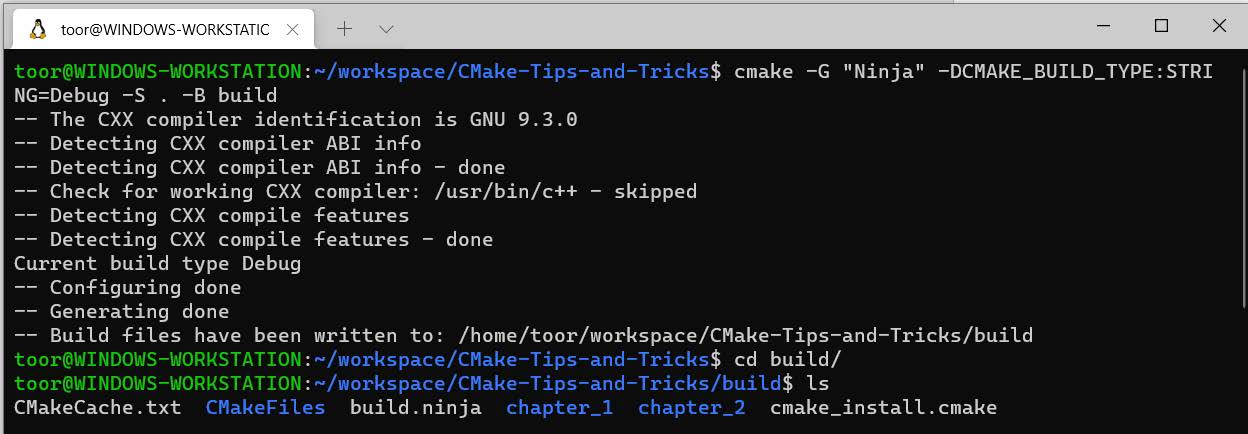
\includegraphics[width=0.8\textwidth]{content/1/chapter2/images/5.jpg}\\
图2.5 检查CMake的Ninja生成器输出
\end{center}

这将导致CMake生成Ninja的构建文件,而不是生成makefile文件。

为了查看环境中可用的生成器类型,可使用\texttt{cmake -{}-help}。可用的生成器将在帮助文本生成器部分的末尾列出:

\begin{center}
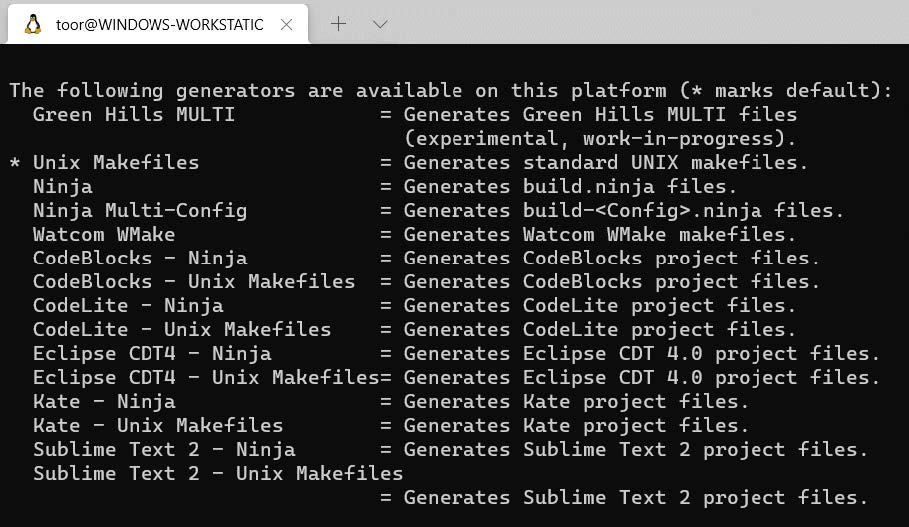
\includegraphics[width=0.6\textwidth]{content/1/chapter2/images/6.jpg}\\
图2.6 可用生成器列表
\end{center}

带有星号的生成器是当前环境的默认值。

\hspace*{\fill} \\ %插入空行
\noindent
\textbf{修改编译器}

CMake中,编译器可以通过CMAKE\_<LANG>\_COMPILER来指定。为了改变编译器,必须在配置命令中提供CMAKE\_<LANG>\_COMPILER。对于C/C++项目,通常修改的是CMAKE\_C\_COMPILER(C编译器)和CMAKE\_CXX\_COMPILER(C++编译器)。编译器标志由CMAKE\_<LANG>\_FLAGS控制。此变量可用于保存与配置无关的编译器标志。

例如,尝试使用g++-10作为C++编译器,但它不是默认编译器:

\begin{tcblisting}{commandshell={}}
cmake -G "Unix Makefiles" -DCMAKE_CXX_COMPILER=/usr/bin/g++-10 -S .  
  -B ./build
\end{tcblisting}

可以看到使用了g++-10,而不是系统默认的编译器g++-9:

\begin{center}
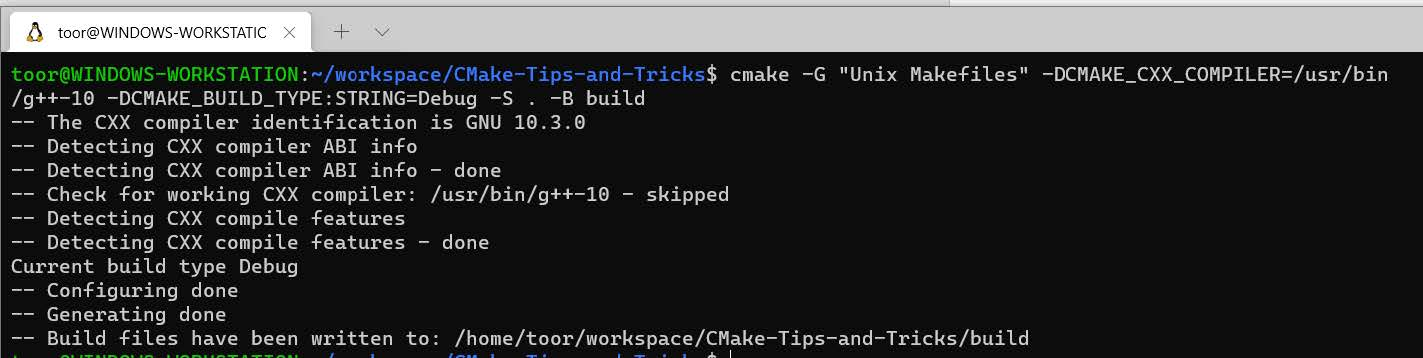
\includegraphics[width=1.\textwidth]{content/1/chapter2/images/7.jpg}\\
图2.7 使用不同的编译器配置项目(g++-10)
\end{center}

没有编译器规范的情况下,CMake更倾向于在这种环境下使用g++-9:

\begin{center}
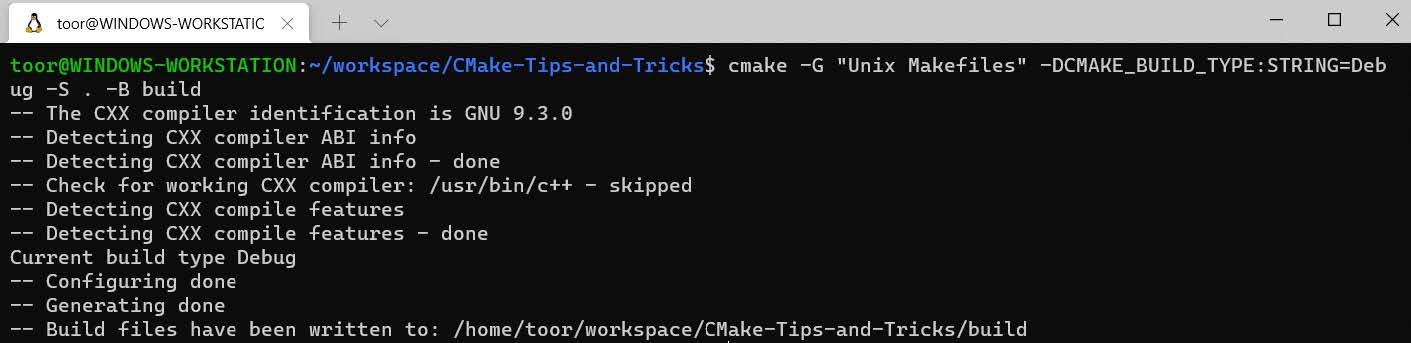
\includegraphics[width=1.\textwidth]{content/1/chapter2/images/8.jpg}\\
图2.8 不使用编译器配置的情况
\end{center}

\hspace*{\fill} \\ %插入空行
\noindent
\textbf{向编译器传递编译标志}

为了演示如何指定编译器标志,假设需要启用警告视为错误。这在gcc工具链中分别用-Wall和-Werror编译器标志控制。因此,需要将这些标志传递给C++编译器:

\begin{tcblisting}{commandshell={}}
cmake -G "Unix Makefiles" -DCMAKE_CXX_FLAGS:STRING="-Wall
  -Werror" - S . B ./build S . -B ./build
\end{tcblisting}

下面的例子中,将标志(-Wall和-Werror)传递给了编译器:

\begin{center}
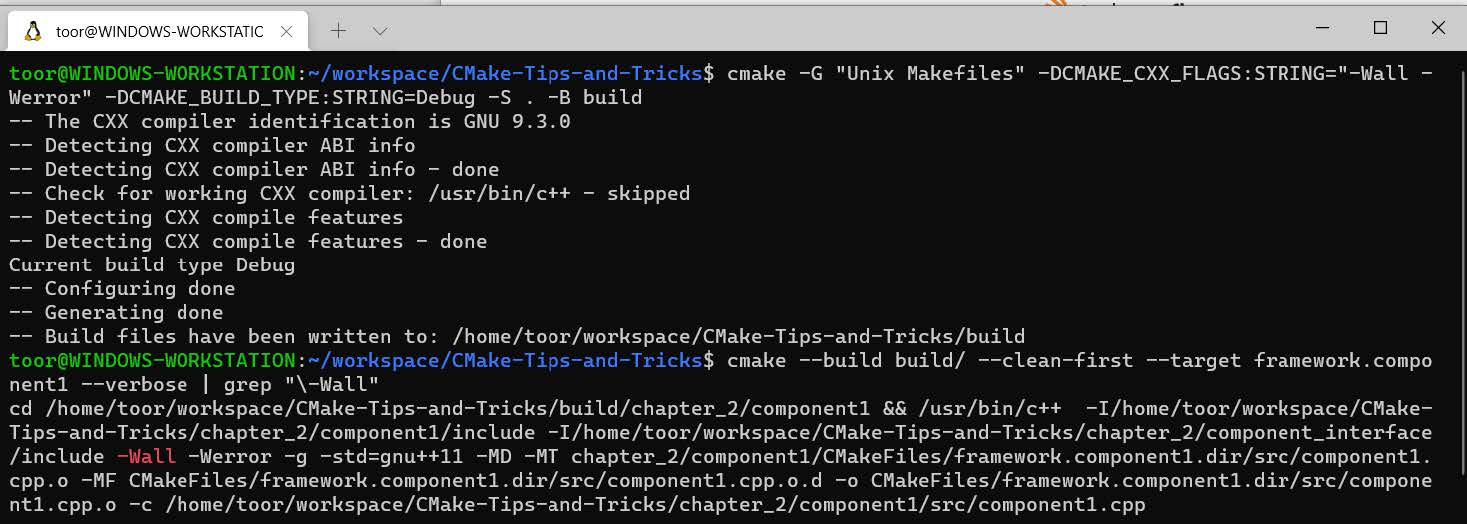
\includegraphics[width=1.\textwidth]{content/1/chapter2/images/9.jpg}\\
图2.9 向C++编译器传递标志
\end{center}

构建标志可以为每个构建类型定制,方法是在它们后面加上大写的构建类型字符串。有四个变量用于四个不同的构建类型,它们对于根据编译器标志指定构建类型非常有用。这些变量中指定的标志只在配置构建类型匹配时有效:

\begin{enumerate}
\item 
CMAKE\_<LANG>\_FLAGS\_DEBUG

\item 
CMAKE\_<LANG>\_FLAGS\_RELEASE

\item 
CMAKE\_<LANG>\_FLAGS\_RELWITHDEBINFO

\item 
CMAKE\_<LANG>\_FLAGS\_MINSIZEREL
\end{enumerate}

若希望只在Release构建中将警告视为错误,可以使用构建类型特定的编译器标志。

下面的示例,演示了如何使用特定于构建类型的编译器标志:

\begin{tcblisting}{commandshell={}}
cmake -G "Unix Makefiles" -DCMAKE_CXX_FLAGS:STRING="-Wall
  -Werror" -DCMAKE_CXX_FLAGS_RELEASE:STRING="-O3" -DCMAKE_BUILD_
  TYPE:STRING=Debug -S . -B ./build
\end{tcblisting}

前面的命令中有一个CMAKE\_CXX\_FLAGS\_RELEASE参数,只有当构建类型为Release时,这个变量中的内容才会传递给编译器。由于构建类型指定为Debug,可以看到传递给编译器的标志中没有-O3标志:

\begin{center}
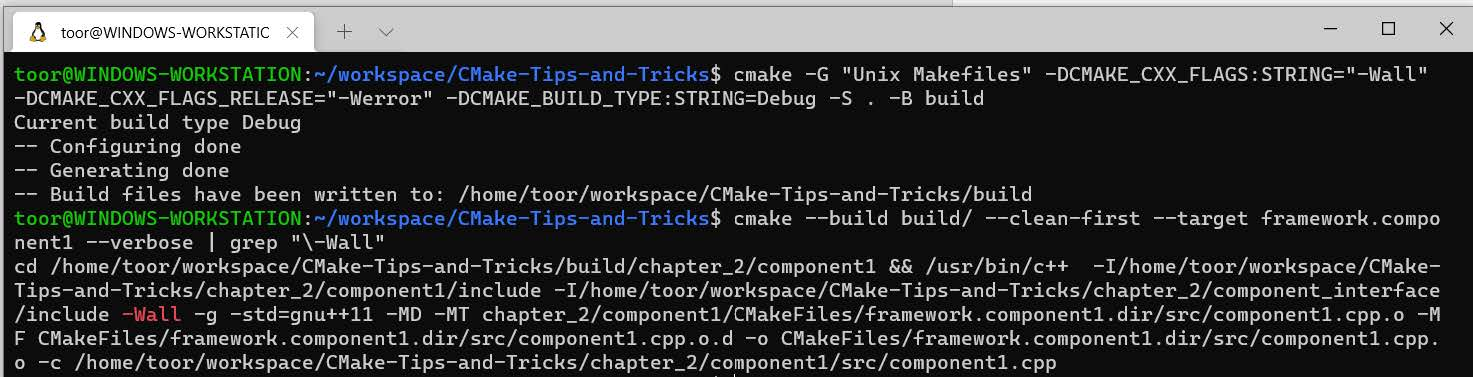
\includegraphics[width=1.\textwidth]{content/1/chapter2/images/10.jpg}\\
图2.10 根据构建类型指定标志——Debug版本中没有-O3标志
\end{center}

图2.10中,CMake发出一个关于指定,但未使用变量的警告,CMAKE\_CXX\_FLAGS\_RELEASE。这确认了CMAKE\_CXX\_FLAGS\_RELEASE没有在Debug构建类型中使用。当构建类型指定为Release时,可以看到-O3标志:

\begin{tcblisting}{commandshell={}}
cmake -G "Unix Makefiles" -DCMAKE_CXX_FLAGS:STRING="-Wall
-Werror" -DCMAKE_CXX_FLAGS_RELEASE:STRING="-O3"
-DCMAKE_BUILD_TYPE:STRING= "Release" -S . -B ./build
\end{tcblisting}

相当于对CMake说,配置位于当前目录的CMake项目,使用“Unix Makefiles”生成器来构建/文件夹。对于所有构建类型,无条件地将-Wall标志传递给编译器。若构建类型是Release,也传递-O3标志。

以下是当构建类型设置为Release时命令的输出:

\begin{center}
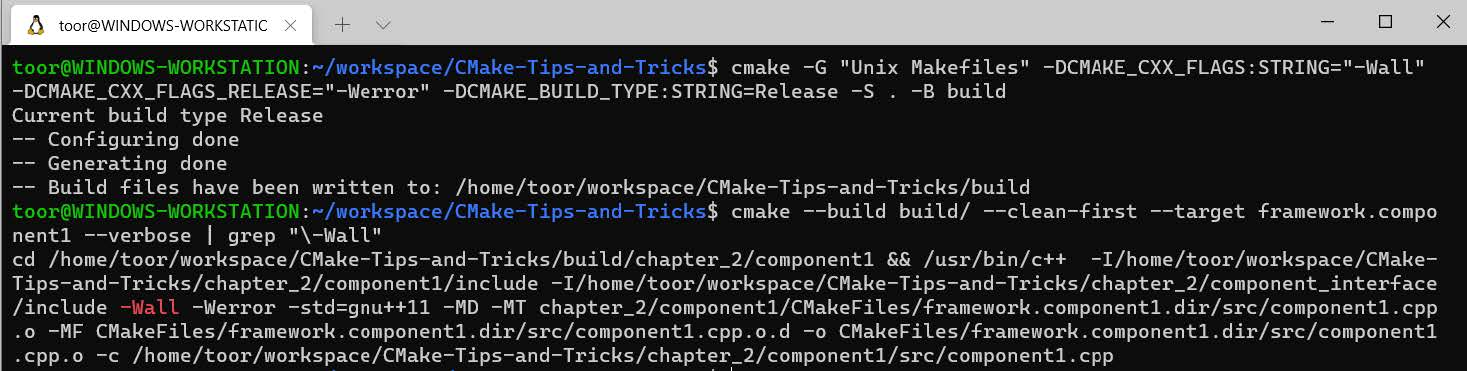
\includegraphics[width=1.\textwidth]{content/1/chapter2/images/11.jpg}\\
图2.11 根据构建类型指定标志——在Release版本中有-O3标志
\end{center}

图2.11中,可以确认-O3标志也传递给了编译器。注意,即使RelWithDebInfo和MinSizeRel也是Release版本,它们与Release版本类型是分开的,因此在CMAKE\_<LANG>\_FLAGS\_RELEASE中指定的标志不适用于它们。

\hspace*{\fill} \\ %插入空行
\noindent
\textbf{缓存变量列表}

可以通过\texttt{cmake -L ./build/}列出所有缓存的变量(参见图2.12)。默认情况下,这不会显示与每个变量关联的高级变量和帮助字符串。也可以使用\texttt{cmake -LAH ./build/}来显示它们。

\begin{center}
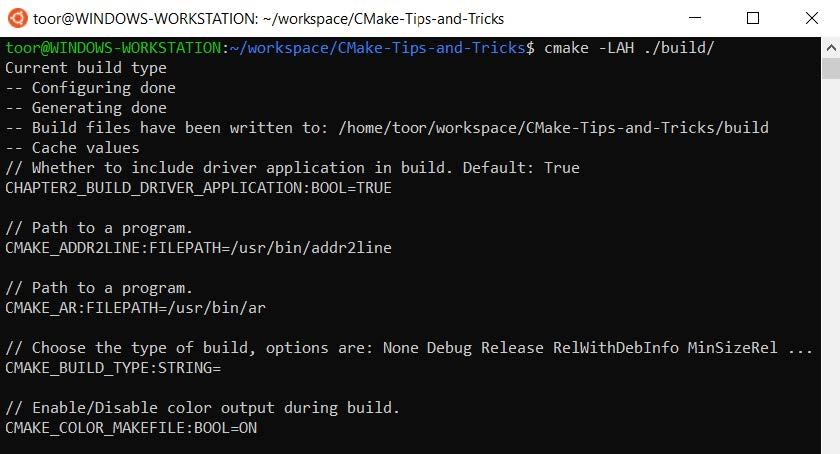
\includegraphics[width=0.8\textwidth]{content/1/chapter2/images/12.jpg}\\
图2.12 CMake转储的缓存变量列表
\end{center}

\hspace*{\fill} \\ %插入空行
\noindent
\textbf{通过CLI构建配置好的项目}

要生成已配置的工程,需要使用\texttt{cmake -{}-build ./build}在构建文件夹中配置的CMake项目。

也可以使用\texttt{cd build \&\& make}进行构建。使用\texttt{cmake -{}-build}的好处是,省去了调用特定于构建系统的命令。在构建CI管道或构建脚本时,可以在不更改构建命令的情况下,更改构建系统生成器。

可以看到\texttt{cmake -{}-build ./build}的输出示例如下所示:

\begin{center}
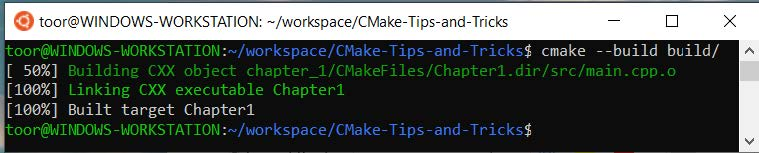
\includegraphics[width=1.\textwidth]{content/1/chapter2/images/13.jpg}\\
图2.13 构建配置好的项目
\end{center}

\hspace*{\fill} \\ %插入空行
\noindent
\textbf{并行构建}

还可以在发出生成命令时,自定义生成时间详细信息。要指定并行构建的任务数,可以在\texttt{cmake -{}-build}中追加\texttt{-{}-parallel <job\_count>}。

要并行构建,请使用\texttt{cmake -{}-build ./build -{}-parallel 2},其中数字2指定了任务数。对于构建系统,建议的任务数最多为每个硬件线程一个作业。多核系统中,还建议至少使用比可用硬件线程数少一个的线程,以避免在构建过程中影响系统的响应能力。

\begin{tcolorbox}[colback=webgreen!5!white,colframe=webgreen!75!black,title=Note]
通常可以在每个硬件线程中使用多个任务,从而获得更快的构建时间,因为构建过程主要受I/O限制,但实际情况可能有所不同,需要进行实验和观察。

此外,某些构建系统(如Ninja)会尝试利用系统中可用的尽可能多的硬件线程,若目标是使用系统中的所有硬件线程,那么为此类构建系统指定任务数就多余了。可以在Linux环境中,使用nproc命令来获取硬件线程计数。
\end{tcolorbox}

在期望在不同环境中调用的命令(如CI/CD脚本和构建脚本)中,不使用环境相关变量的固定值,这是一个很好的实践。下面是一个使用nproc动态确定并行任务数量的构建命令示例:

\begin{tcblisting}{commandshell={}}
cmake --build ./build/ --parallel $(($(nproc)-1))
\end{tcblisting}

观察不同的任务数如何影响构建时间,将使用时间工具来测试每次命令调用的时间。环境如下:

\begin{itemize}
\item 
OS: Ubuntu 20.04.3 LTS (Focal Fossa)

\item 
CPU: AMD Ryzen Threadripper 1950X 16-Core Processor (32线程)

\item 
RAM: 32 GB
\end{itemize}

对于一个任务(\texttt{-{}-parallel 1}),构建时间如下所示:

\begin{center}
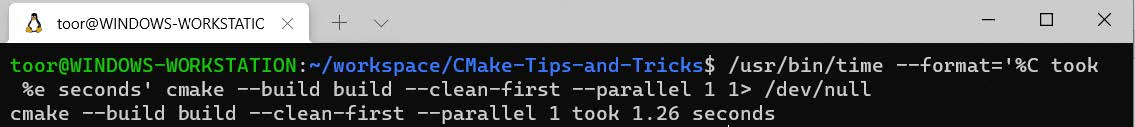
\includegraphics[width=1.\textwidth]{content/1/chapter2/images/14.jpg}\\
图2.14 一个任务的并行构建时间结果
\end{center}

两个任务(\texttt{-{}-parallel 2})的构建时间结果如下:

\begin{center}
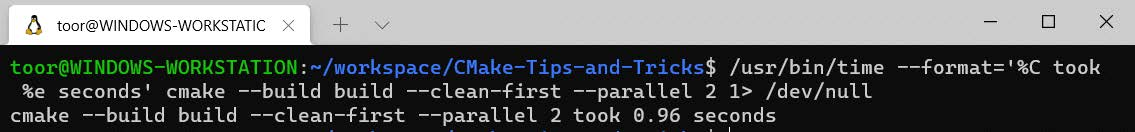
\includegraphics[width=1.\textwidth]{content/1/chapter2/images/15.jpg}\\
图2.15 两个任务的并行构建时间结果
\end{center}

三个任务(\texttt{-{}-parallel 3})的构建时间结果如下:

\begin{center}
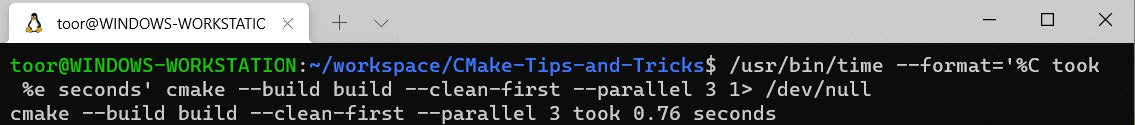
\includegraphics[width=1.\textwidth]{content/1/chapter2/images/16.jpg}\\
图2.16 三个任务的并行构建时间结果
\end{center}

四个任务(\texttt{-{}-parallel 4})的构建时间结果如下:

\begin{center}
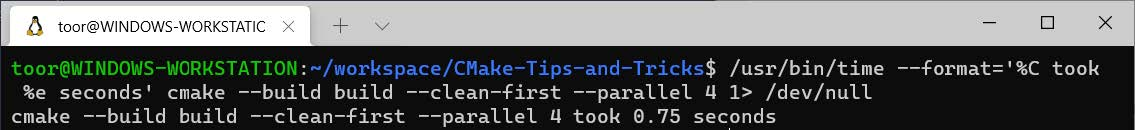
\includegraphics[width=1.\textwidth]{content/1/chapter2/images/17.jpg}\\
图2.17 四个任务的并行构建时间结果
\end{center}

即使是一个非常简单的项目,也可以清楚地看到多个任务并行可以减少构建时间。从一个作业到两个任务减少了0.3秒的构建时间,而从两个任务到三个任务则减少了0.2秒。但是,从3个作业到4个任务只会产生0.01秒的差异,这意味着已经达到了这个项目的构建并行性的极限,增加更多的工作将不会在构建时间上实现显著的差异。

\hspace*{\fill} \\ %插入空行
\noindent
\textbf{只构建特定的目标}

通常,CMake将构建已配置的所有可用目标。由于构建所有目标并不总是理想的,CMake允许通过-{}-target子选项构建目标的子集,子选项可以指定多次:

\begin{tcblisting}{commandshell={}}
cmake --build ./build/ --target "ch2_framework_component1"
--target "ch2_framework_component2"
\end{tcblisting}

该命令将构建范围限制为ch2\_framework\_component1和ch2\_framework\_component2目标。若这些目标也依赖于其他目标,它们也会构建。

\hspace*{\fill} \\ %插入空行
\noindent
\textbf{构建之前删除以前的构建}

若想要运行一个干净的构建,首先就要删除之前的构建。为此,可以使用-{}-clean-first子选项。此子选项将调用一个特殊的目标,该目标清除由构建过程生成的所有构件(例如,调用make clean)。

下面是一个示例,说明如何对名为build的构建文件夹执行此操作:

\begin{tcblisting}{commandshell={}}
cmake --build ./build/ --clean-first
\end{tcblisting}

\hspace*{\fill} \\ %插入空行
\noindent
\textbf{调试构建过程}

正如在前面的向编译器传递标志一节中所做的那样,可能希望检查构建过程中使用哪些参数调用了哪些命令。-{}-verbose指示CMake以verbose模式调用所有构建命令,前提是该命令支持verbose模式。这使我们能够轻松地调试编译和链接错误。

要在verbose模式下构建名为build的文件夹,可以使用\texttt{-{}-build}:

\begin{tcblisting}{commandshell={}}
cmake --build ./build/ --verbose
\end{tcblisting}

\hspace*{\fill} \\ %插入空行
\noindent
\textbf{将命令行参数传递给构建工具}

若需要将参数传递给底层构建工具,可以在命令的末尾加上\texttt{-{}-},并输入给定的参数:

\begin{tcblisting}{commandshell={}}
cmake --build ./build/ -- --trace
\end{tcblisting}

-{}-trace将直接传递给构建工具,例子中就是make。这将使make为构建每个文件的编译和连接输出跟踪信息。

\hspace*{\fill} \\ %插入空行
\noindent
\textbf{通过CLI安装项目}

CMake允许在环境中进行安装,CMake代码必须使用\texttt{install()}指令来指定当调用\texttt{cmake -{}-install}(或构建系统等效)时安装什么。chapter2的内容已经以这样的方式配置用于说明指令。我们将在第4章中学习如何使CMake目标可安装。

\texttt{cmake -{}-install}需要一个已经配置和生成的项目,执行\texttt{cmake -{}-install <project\_binary\_dir>}来安装工程。我们的例子中,build作为项目二进制目录,所以<project\_binary\_dir>将为build。

示例输出如下图所示:

\begin{center}
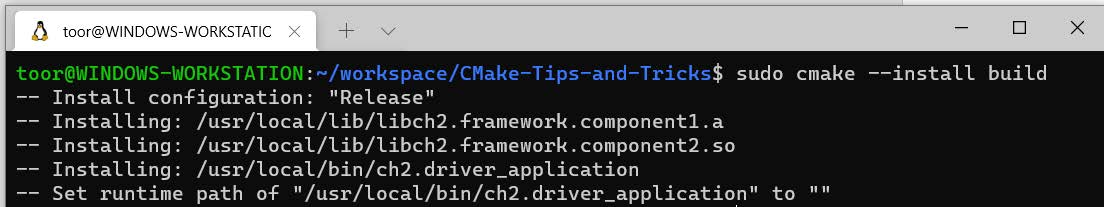
\includegraphics[width=1.\textwidth]{content/1/chapter2/images/18.jpg}\\
图2.18 安装工程
\end{center}

不同环境的默认安装目录不同。对于类Unix环境,默认为\texttt{/usr/local},而在Windows环境中,默认为\texttt{C:/Program Files}。

\begin{tcolorbox}[colback=webgreen!5!white,colframe=webgreen!75!black,title=Tip]
在尝试安装项目之前,必须已经构建了项目。

为了能够成功安装项目,必须拥有适当的权限来写入安装目标目录。
\end{tcolorbox}

\hspace*{\fill} \\ %插入空行
\noindent
\textbf{修改默认安装路径}

要更改默认安装目录,可以指定的-{}-prefix参数,如下所示:

\begin{tcblisting}{commandshell={}}
cmake --install build --prefix /tmp/example
\end{tcblisting}

将安装目录指定为/tmp/example,使用\texttt{cmake -{}-install}后,/tmp/example目录下的内容如下图所示:

\begin{center}
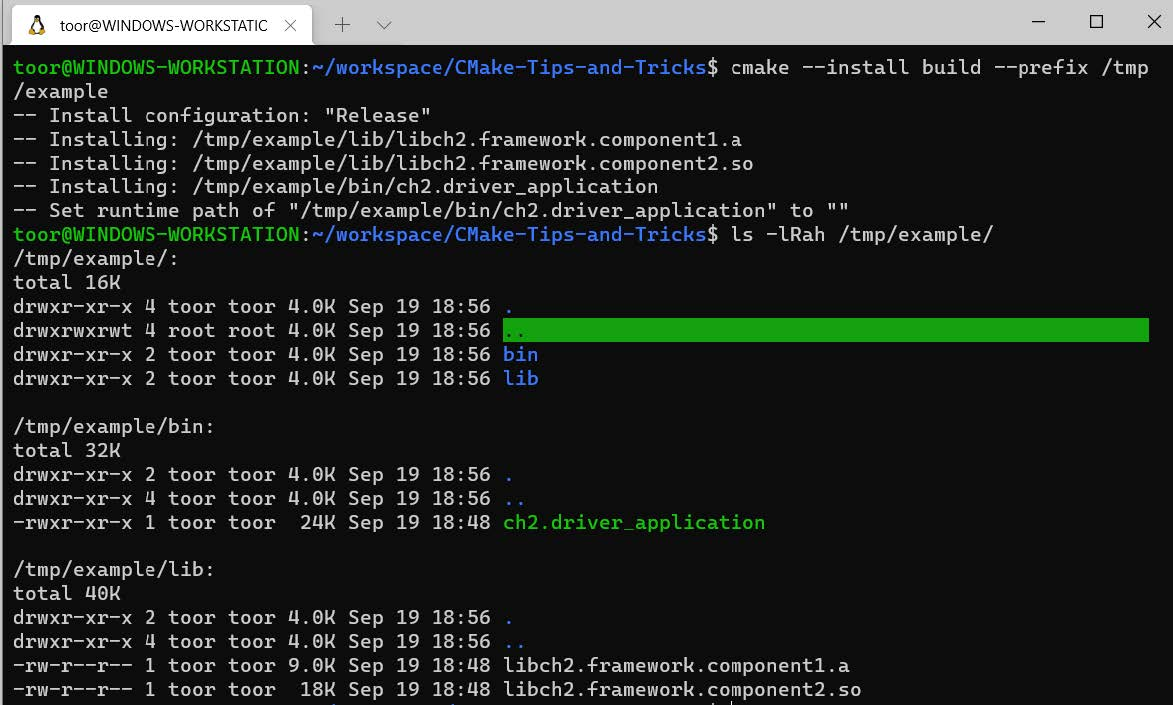
\includegraphics[width=0.8\textwidth]{content/1/chapter2/images/19.jpg}\\
图2.19 将项目安装到不同的路径
\end{center}

可以看到,安装根目录成功更改为/tmp/example。

\hspace*{\fill} \\ %插入空行
\noindent
\textbf{安装时瘦身二进制文件}

软件世界中,构建工件通常与一些额外的信息捆绑在一起,例如:调试所需的符号表。这些信息在最终产品时可能不是必需的,并且可能会极大地增加二进制大小。若希望减少最终产品的存储空间,瘦身二进制文件可能是一个不错的选择。瘦身的另一个好处是,这会使逆向工程二进制文件变得更加困难,因为从二进制文件中剥离了基本的符号信息。

CMake的\texttt{-{}-install}允许在安装操作时瘦身二进制文件。可以通过在-{}-install中使用-{}-strip选项来启用:

\begin{tcblisting}{commandshell={}}
cmake --install build --strip
\end{tcblisting}

下面的示例中,可以观察未瘦身和瘦身的二进制文件之间的大小差异。注意,瘦身静态库有一些限制,CMake默认情况下不会执行:

\begin{center}
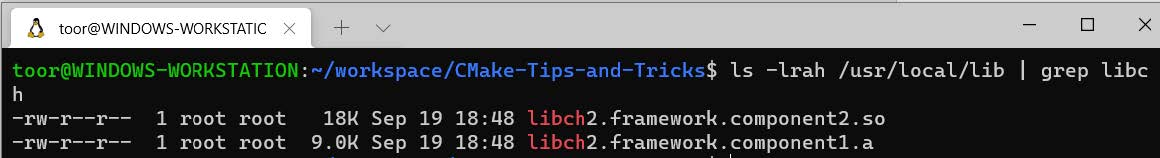
\includegraphics[width=1.\textwidth]{content/1/chapter2/images/20.jpg}\\
图2.20 工件大小(未瘦身)
\end{center}

使用瘦身的(\texttt{cmake - install build -{}-strip})二进制文件,大小差异如下图所示:

\begin{center}
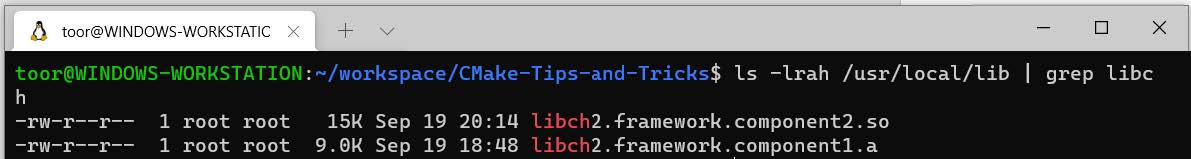
\includegraphics[width=1.\textwidth]{content/1/chapter2/images/21.jpg}\\
图2.21 工件大小(已瘦身)
\end{center}

\hspace*{\fill} \\ %插入空行
\noindent
\textbf{安装特定组件(基于组件的安装)}

若项目在\texttt{install()}中使用了CMake的COMPONENT特性,可以通过指定组件名称来安装特定的组件。组件特性允许将安装分离为子部分,为了说明这个功能,chapter2示例构造成两个组件,分别是库和可执行文件。

为了安装特定的组件,\texttt{cmake -{}-install}需要附加-{}-component参数:

\begin{tcblisting}{commandshell={}}
cmake --install build --component executables
\end{tcblisting}

下面是一个示例:

\begin{center}
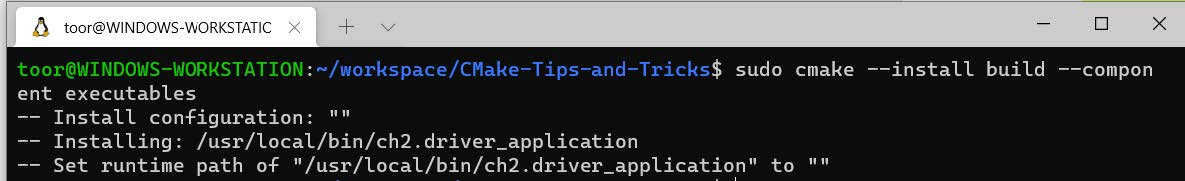
\includegraphics[width=1.\textwidth]{content/1/chapter2/images/22.jpg}\\
图2.22 只安装特定的组件
\end{center}

\hspace*{\fill} \\ %插入空行
\noindent
\textbf{安装特定的配置(仅用于多配置生成器)}

有些生成器支持同一个构建配置的多个配置(例如,Visual Studio)。对于这种类型的生成器,\texttt{-{}-install}选项提供了一个\texttt{-{}-config}参数来指定要安装的二进制文件配置。

这里有一个例子:

\begin{tcblisting}{commandshell={}}
cmake --install build --config Debug
\end{tcblisting}

\begin{tcolorbox}[colback=webgreen!5!white,colframe=webgreen!75!black,title=Note]
示例中使用的命令参数非常长且明确,显式地指定参数允许我们在每次运行中获得一致的结果,无论在哪个环境中运行命令。若没有-G参数,CMake将默认使用环境首选的构建系统生成器。我们的座右铭是:显式总是比隐式好,前者使我们的意图更加清晰,也使CMake代码更容易维护。
\end{tcolorbox}

我们已经介绍了CMake命令行用法的基本原理,继续学习其他可用的交互形式——CMake的图形界面。











